\chapter{Introduction}\label{introduction}

The \emph{AMBA APB v2.0} bus protocol - commonly referred to as APB4 - 
defines a low-cost interface that is optimized for minimal power
consumption and reduced interface complexity. To enable a single APB4
Master to communicate with \emph{multiple} APB4 Slaves (Peripherals) via
a common bus, certain signals require multiplexing -- the Roa Logic APB4
Multiplexer is a fully configurable \& parameterized IP to provide this
functionality as shown below:

\begin{figure}[th]
	\centering
	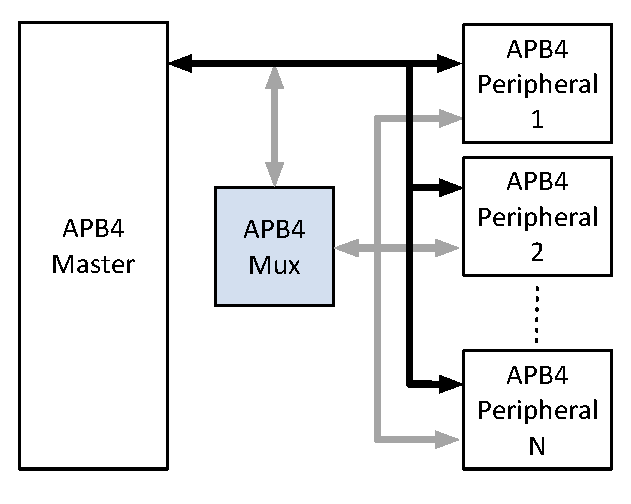
\includegraphics{assets/img/APB4-Mux-Sys}
	\caption{APB4 Multiplexer System}
	\label{fig:apb4-mux-sys}
\end{figure}

\section{Features}\label{features}

\begin{itemize}
\item
  Full support for \emph{APB version 2.0} (APB4) protocol
\item
  Fully parameterized IP with:
  \begin{itemize}
  \item
    User Configurable number of peripherals supported
  \item
    User Configurable address and data widths
  \end{itemize}
\item
  Support for user defined address mapping per peripheral
\end{itemize}
